\documentclass[11pt,a4paper]{article}
\usepackage[utf8]{inputenc}
\usepackage[T1]{fontenc}
\usepackage[english]{babel}
\usepackage{geometry}
\geometry{a4paper, margin=2.5cm}
\usepackage{graphicx}
\usepackage{amsmath,amssymb}
\usepackage{booktabs}
\usepackage{hyperref}
\usepackage{xcolor}
\usepackage{enumitem}
\usepackage{float}

% Custom colors
\definecolor{darkblue}{RGB}{0,51,102}
\definecolor{lightgray}{RGB}{240,240,240}

% Section formatting
\usepackage{titlesec}
\titleformat{\section}{\Large\bfseries\color{darkblue}}{\thesection}{1em}{}
\titleformat{\subsection}{\large\bfseries\color{darkblue}}{\thesubsection}{1em}{}

% Header and footer
\usepackage{fancyhdr}
\pagestyle{fancy}
\fancyhf{}
\rhead{\footnotesize Bantou 2027 — ANP Drug Discovery}
\lhead{\footnotesize PHC Program}
\cfoot{\thepage}

\hypersetup{
    colorlinks=true,
    linkcolor=darkblue,
    filecolor=darkblue,
    urlcolor=darkblue,
    citecolor=darkblue
}

\title{\textbf{Hybrid Quantum-Classical Machine Learning for\\
African Natural Products Drug Discovery:\\
A Computational Framework for Antimalarial Development}}

\author{
    \textbf{Programme PHC BANTOU 2027}\\[0.5em]
    \normalsize France--Cameroon Scientific Cooperation\\[1em]
    \normalsize \textit{Franco-Cameroonian Joint Research Proposal}\\[0.5em]
    \normalsize \textit{Draft version V2 — 6 October 2026}
}

\date{6 October 2026}

\begin{document}

\thispagestyle{empty}
\maketitle

\begin{abstract}
\noindent
African natural products (ANPs) represent a vast, structurally complex chemical space with unique antimalarial potential, yet they remain underexplored by conventional drug discovery methods. This Franco-Cameroonian collaborative project proposes to develop and validate hybrid quantum-classical machine learning architectures specifically designed to capture the stereochemical and three-dimensional structural complexity of ANPs that classical fingerprints miss. Building on five completed computational studies (chemical space exploration, molecular dynamics validation, quantum-inspired representations, Monte Carlo optimization, and graph neural networks), we will implement true quantum machine learning methods to address the scaffold generalization bottleneck observed in classical models. The project integrates computational chemistry, quantum computing, machine learning, and ethnobotanical knowledge to prioritize ANP-derived antimalarial candidates while ensuring computational accessibility for African research institutions. Our approach honors the cultural heritage of traditional African medicine and creates a sustainable framework for ANP-based drug discovery with direct relevance to malaria-endemic regions.

\vspace{0.5em}
\noindent\textbf{Keywords:} African Natural Products, Antimalarial Drug Discovery, Quantum Machine Learning, Molecular Encoding, Scaffold Generalization, Computational Accessibility, Franco-Cameroonian Collaboration
\end{abstract}

\clearpage
\tableofcontents
\clearpage

\section{Scientific Background and Rationale}

\subsection{The Malaria Challenge in Africa}

Malaria remains a devastating public health burden in sub-Saharan Africa. According to the WHO \textit{World Malaria Report 2025}, the WHO African Region carried about 94\% of global malaria cases (265 million of an estimated 282 million cases) and about 95\% of malaria deaths (579\,000 of an estimated 610\,000 deaths) in 2024 \cite{who2025}. The emergence of resistance to frontline antimalarial drugs (chloroquine, sulfadoxine-pyrimethamine, artemisinin-based combination therapies) threatens decades of progress in malaria control. Novel antimalarial scaffolds with multi-target mechanisms are urgently needed to circumvent resistance evolution and provide sustainable therapeutic options for malaria-endemic populations.

\subsection{African Natural Products: An Underexplored Resource}

African natural products offer several unique advantages for antimalarial drug discovery:

\begin{itemize}[leftmargin=1.5em]
    \item \textbf{Structural Complexity:} ANPs possess high molecular complexity (Fsp$^3$ often $>$ 0.5, multiple stereocenters, polycyclic scaffolds) that distinguish them from typical synthetic drug-like compounds (Fsp$^3$ $\sim$ 0.3--0.4) \cite{lovering2009}.
    \item \textbf{Ethnobotanical Heritage:} Traditional African medicine has documented antimalarial use of plants such as \textit{Cryptolepis sanguinolenta}, \textit{Enantia chlorantha}, \textit{Nauclea latifolia}, and \textit{Artemisia annua} for centuries, providing evidence-based starting points for scientific investigation \cite{bero2009}. The AfroDb collection provides freely downloadable three-dimensional structures for 1\,008 natural products from African medicinal plants, spanning a wide range of reported biological activities including antimalarial \cite{ntiekang2013}.
    \item \textbf{Evolutionary Polypharmacology:} Secondary metabolites in ANPs evolved to interact with multiple biological targets, offering inherent multi-target activity that may slow resistance development.
    \item \textbf{Chemical Diversity:} ANPs span diverse chemical families including indole alkaloids, prenylated flavonoids, quassinoids, and sesquiterpene lactones, expanding chemical space beyond conventional screening libraries.
\end{itemize}

\subsection{Computational Limitations of Classical Methods}

Our preliminary work (Studies 1--5, described below) has revealed fundamental limitations of classical computational methods when applied to ANPs:

\begin{enumerate}[leftmargin=1.5em]
    \item \textbf{Static Docking Failures (Studies 1--2):} Molecular docking on rigid protein structures (GNINA \cite{mcnutt2021}) cannot capture ANP conformational flexibility, leading to 87.5\% disagreement between docking scores and molecular dynamics-derived binding affinities (Study 2).
    \item \textbf{Loss of Stereochemistry (Study 3):} Classical fingerprints (ECFP4 \cite{rogers2010}) and quantum-inspired methods encode flattened molecular representations, losing critical stereochemical and three-dimensional information that defines ANP bioactivity.
    \item \textbf{Scaffold Generalization Bottleneck (Study 5):} Graph neural networks (GNNs) based on 1-Weisfeiler-Lehman (1-WL) message passing fail on ANP scaffold splits (AUC = 0.649 vs. ECFP4-RF baseline 0.689), unable to distinguish stereoisomers or capture non-local structural patterns in high-Fsp$^3$ molecules \cite{morris2019}.
\end{enumerate}

\subsection{Quantum Machine Learning as a Solution}

Hybrid quantum-classical machine learning offers a principled approach to overcome these limitations by:

\begin{itemize}[leftmargin=1.5em]
    \item \textbf{Direct Structural Encoding:} Quantum molecular state encoding (QMSE) preserves bond orders, stereochemistry (E/Z, R/S), and 3D topology through quantum circuit representations in $2^n$ Hilbert space, consistent with recent work on molecular encodings for quantum machine learning \cite{boy2025,havlicek2019}.
    \item \textbf{Non-Local Feature Learning:} Quantum feature extractors (QFE) capture long-range structural correlations beyond k-hop GNN neighborhoods, addressing the 1-WL expressivity bottleneck \cite{morris2019}.
    \item \textbf{Computational Efficiency:} Quantum kernel transfer (QKT) enables accurate predictions on large datasets after quantum pre-training on small ANP-rich subsets, making the method accessible to resource-limited African laboratories. Hardware demonstrations to date remain exploratory and must be interpreted cautiously on noisy intermediate-scale quantum (NISQ) devices \cite{preskill2018,kim2023}.
\end{itemize}

\subsection{Franco-Cameroonian Complementarity}

This collaboration leverages unique complementary expertise:

\begin{itemize}[leftmargin=1.5em]
    \item \textbf{French Team:} Advanced computational infrastructure, quantum computing access (IBM Quantum, cloud-based NISQ devices), machine learning expertise, and established computational chemistry pipelines.
    \item \textbf{Cameroonian Team:} Ethnobotanical knowledge, governance of ANP compound libraries and metadata, traditional medicine expertise, botanical specimen identification, local deployment of CPU-only inference workflows, and direct connection to malaria-endemic populations informing translational priorities.
\end{itemize}

Together, we will create a sustainable ANP drug discovery pipeline that honors African cultural heritage while advancing quantum computing applications in medicinal chemistry.

\section{Preliminary Work: Studies 1--5 Foundation}

Our team has completed five computational studies that establish the scientific foundation and reveal the computational challenge that this proposal addresses. (A sixth ongoing study on phenotype--mode-of-action mapping is out of scope for this proposal and will not be reported here.)

\subsection{Study 1: Hybrid Library Construction and Chemical-Space Exploration (Completed)}

\textbf{Objective:} Generate and characterize a hybrid ANP-synthetic compound library for antimalarial screening.

\textbf{Methods:}
\begin{itemize}
    \item 396 African natural product seeds from ANPDB/AfroDb databases \cite{ntiekang2013}
    \item Enumeration protocol: scaffold hopping, ring expansion/contraction, bioisosteric replacement
    \item Final library: 65,856 compounds with 69.3\% scaffold conservation of ANP privileged cores \cite{bemis1996}
\end{itemize}

\textbf{Key Results:}
\begin{itemize}
    \item 92.6\% of library molecules unreachable by ECFP4 similarity search (Tanimoto $<$ 0.7)
    \item Top-20 candidates (Set A) selected by multi-parameter optimization (MPO 0.515--0.550)
    \item All candidates show selectivity index $>$ 10 (antimalarial vs. cytotoxicity)
    \item External validation: DEKOIS 2.0 benchmark \cite{bauer2013}, Medicines for Malaria Venture (MMV) end-point enrichment, redocking RMSD $<$ 2.0\,\AA
\end{itemize}

\textbf{Status:} Manuscript completed and validated (DEKOIS 2.0, MMV, redocking); Zenodo DOI 10.5281/zenodo.22696778 (public); submission to a specialist journal in progress following an editorial decision in September 2026.

\subsection{Study 2: Molecular Dynamics Validation (Completed)}

\textbf{Objective:} Validate docking predictions through all-atom molecular dynamics simulations.

\textbf{Methods:}
\begin{itemize}
    \item 16 protein--ligand systems: two ligand series $\times$ PfDHFR/PfCRT $\times$ wild-type/mutant states
    \item OpenFF 2.2.0 AM1-BCC force field + CHARMM36m/TIP3P explicit solvent
    \item 25\,ns production trajectories with MM-PBSA binding free energy calculations
\end{itemize}

\textbf{Key Results:}
\begin{itemize}
    \item 87.5\% estimand divergence: docking scores do not predict MD-derived $\Delta G_{\text{bind}}$
    \item Divergence attributed to ANP conformational flexibility and solvation effects
    \item Class A* leads (three series, internal IDs retained in the companion manuscript) show broad target profiles and mutation resilience
    \item GNINA CNN validation \cite{mcnutt2021}: 100\% agreement on Class-A ligand ranking
\end{itemize}

\textbf{Status:} Companion manuscript (current revision) technically ready for submission to a specialist journal; main text and supporting information complete, submission package assembled.

\subsection{Study 3: Quantum-Inspired Representations (Completed)}

\textbf{Objective:} Evaluate quantum-inspired encodings (quantum kernels, topological features) for ANP activity prediction.

\textbf{Methods:}
\begin{itemize}
    \item Quantum kernel states (QKS) from ECFP4 features mapped to RBF/Matern/polynomial kernels
    \item Topological fingerprints (TFP) and topological neural encodings (TNE) via persistent homology
    \item Benchmark dataset: 19,849 molecules with antimalarial activity labels (see \S\ref{sec:data} for provenance)
\end{itemize}

\textbf{Key Results --- Honest Negative:}
\begin{itemize}
    \item \textbf{No quantum advantage:} QKS $\approx$ RBF kernel (0.8876 vs. 0.8819), both underperform ECFP4-RF baseline (0.9475)
    \item Topological features (H$_0$, H$_1$ Betti numbers) capture ANP ring topology but are insufficient for full activity prediction
    \item \textbf{Root cause:} Quantum-inspired methods encode \textit{flattened classical fingerprints}, losing ANP stereochemistry and 3D structure
\end{itemize}

\textbf{Status:} Manuscript claim-calibrated after internal review; submission package ready, targeting the \textit{Journal of Computer-Aided Molecular Design (JCAMD)}.

\subsection{Study 4: Monte Carlo Exploration (Completed)}

\textbf{Objective:} Compare random sampling vs. Monte Carlo tree search (MCTS) for multi-objective optimization.

\textbf{Key Results:}
\begin{itemize}
    \item Random sampling (AUC 0.6724) outperforms MCTS (0.6649) on scaffold-based benchmark
    \item Earlier exploratory Pareto-front artifacts were distinguished from the validated scalar benchmark before any claim was made
    \item Manuscript targeted at a specialist journal of computer-aided molecular design
\end{itemize}

\subsection{Study 5: Graph Neural Networks (Completed)}

\textbf{Objective:} Evaluate GNN architectures for ANP activity prediction and scaffold generalization.

\textbf{Methods:}
\begin{itemize}
    \item GNN architectures (GCN, GAT, GraphSAGE) trained on molecular graphs with phenotypic mode-of-action annotations; evaluation follows standard molecular-ML benchmark practice \cite{wu2018}
    \item Scaffold split using Bemis--Murcko decomposition \cite{bemis1996} (external validation)
\end{itemize}

\textbf{Key Results --- The Scaffold Generalization Bottleneck:}
\begin{itemize}
    \item \textbf{Random split:} GNN performs competitively (AUC $\sim$ 0.85)
    \item \textbf{Scaffold split:} GNN underperforms (0.649) vs. ECFP4-RF baseline (0.689)
    \item \textbf{Root cause:} 1-WL message passing cannot distinguish stereoisomers, cis/trans configurations, or ring fusions in high-Fsp$^3$ ANPs \cite{morris2019}
    \item Topological fusion provides modest complementarity but does not overcome the bottleneck
\end{itemize}

\textbf{Status:} Manuscript claim-calibrated and targeting \textit{RSC Digital Discovery}.

\subsection{Summary: From Studies 1--5 to the Present Project}

Studies 1--5 systematically reveal that:
\begin{enumerate}
    \item ANPs possess unique structural complexity (high Fsp$^3$, stereocenters, 3D topology)
    \item Classical methods (ECFP4 \cite{rogers2010}, GNNs \cite{morris2019}) lose critical ANP structural information
    \item Quantum-inspired approaches (Study 3) do not solve the problem because they encode classical features
    \item \textbf{True quantum machine learning with direct molecular encoding is needed} --- the object of the present proposal
\end{enumerate}

\section{Proposed Research}

\subsection{Central Hypothesis}

\textbf{Hybrid quantum-classical machine-learning architectures that encode ANP topology and stereochemistry directly at the quantum-circuit level improve scaffold-generalization AUC by at least $\Delta$AUC $\geq 0.02$ over the classical ECFP4-RF baseline (AUC = 0.689), with the largest gains in the highest African-Chemotype Structural Index (ACSI) quartile; architectures that merely re-encode classical fingerprints will fail to exceed this margin.}

This hypothesis is falsifiable under the estimands and decision rules pre-declared in \S\ref{sec:stats}. It explicitly includes the honest-negative case: if no architecture meets the margin, the result identifies where quantum enhancement does and does not pay off on ANP chemical space.

\subsection{Specific Aims}

\subsubsection{Aim 1: Quantum Molecular State Encoding (QMSE) for ANPs --- Guaranteed scope}

\textbf{Objective:} Develop quantum circuit representations that preserve ANP stereochemistry, bond topology, and 3D geometry.

\textbf{Approach:}
\begin{itemize}
    \item Implement BondOrderMatrix encoding: bond orders (1/1.5/2/3), stereochemistry (E/Z: negative bond order; R/S: negative diagonal) following Boy et al.\ \cite{boy2025}
    \item Coulomb matrix encoding for 3D geometry (atomic distances, nuclear charges) \cite{rupp2012}
    \item Map molecular features to quantum states in $2^n$ Hilbert space via variational quantum circuits
\end{itemize}

\textbf{Validation:}
\begin{itemize}
    \item Kernel target alignment: Does quantum kernel $K(A,B)$ correlate with structural similarity better than ECFP4 Tanimoto similarity \cite{rogers2010}?
    \item Feature attribution: Which ANP structural features (stereocenters, ring fusions, macrocycles) drive quantum vs.\ classical predictions?
\end{itemize}

\textbf{Success Criterion (aligned on the full benchmark):} Mean kernel target alignment on the ACSI-stratified ANP-rich subset exceeds the ECFP4 Tanimoto baseline by $\Delta\text{alignment} \geq +0.05$, with a bootstrap 95\% CI excluding zero, on the Study 3 benchmark ($n = 19{,}849$) and its ANP-rich subset. Set A ($n = 20$) is used only as a feasibility demonstration (proof of concept), not as the inferential sample.

\subsubsection{Aim 2: Hybrid Quantum-Classical Architectures (QKT guaranteed; QFE and Q-GNN stretched)}

\textbf{Objective:} Design three architectures balancing quantum expressivity and computational feasibility. The guaranteed core of the project is Aim 1 (QMSE) + the QKT architecture (this aim) + Aim 3 (ACSI stratification); QFE training, the Q-GNN, and the full 10k external validation are \textbf{stretched objectives} subject to Risk 3 (see \S\ref{sec:risk}).

\textbf{Architecture 1: Quantum Feature Extractor (QFE)}
\begin{itemize}
    \item Input: Molecular graph or fingerprint
    \item Quantum layer: Trainable parametrized quantum circuit (PQC) with entangling gates
    \item Classical layer: Feedforward neural network for activity prediction
    \item Training: End-to-end backpropagation with PQC parameter optimization
\end{itemize}

\textbf{Architecture 2: Quantum Graph Neural Network (Q-GNN) --- Stretched}
\begin{itemize}
    \item GNN message passing for local features (k-hop neighborhoods) \cite{morris2019}
    \item Quantum layer processes global graph embedding in $2^n$ Hilbert space
    \item Captures non-local ANP structural patterns beyond 1-WL expressivity
    \item Addresses the Study 5 scaffold generalization bottleneck
\end{itemize}

\textbf{Architecture 3: Quantum Kernel Transfer (QKT) --- Guaranteed}
\begin{itemize}
    \item Stage 1: Quantum kernel on ANP-rich subsets (Study 1 Set A plus stratified Study 3 ANP subset) --- $O(n^2)$ kernel entries
    \item Stage 2: Transfer learned features to a classical neural network
    \item Stage 3: Fine-tune on the full Study 3 benchmark ($n = 19{,}849$) --- $O(n)$ inference
    \item Computational efficiency: Enables CPU-only inference for African laboratories (to be demonstrated locally in Cameroon, see \S\ref{sec:cmwork})
\end{itemize}

\subsubsection{Aim 3: ANP-Stratified Evaluation --- Guaranteed scope}

\textbf{Objective:} Determine for which ANP structural classes quantum enhancement provides advantage, equivalence, or no benefit.

\textbf{African-Chemotype Structural Index (ACSI):} We define the ACSI \textit{a priori} as a purely molecular-descriptor score. Botanical origin is \textit{not} part of the score (to avoid circularity); it is used as a separate stratification variable. Weights are fixed before any model is trained:

\begin{equation}
\text{ACSI} = 0.40\,\text{Fsp}^3 + 0.30\,\min\!\left(\frac{n_{\text{stereo}}}{6}, 1\right) + 0.30\,\min\!\left(\frac{n_{\text{ring atoms}}}{15}, 1\right)
\label{eq:acsi}
\end{equation}

where Fsp$^3$ is the fraction of sp$^3$-hybridized carbons, $n_{\text{stereo}}$ the number of tetrahedral/double-bond stereocenters, and $n_{\text{ring atoms}}$ the number of heavy atoms in the Bemis--Murcko scaffold \cite{bemis1996,lovering2009}. All descriptors are computed with RDKit; quartile cut-points are computed once on the frozen benchmark (see \S\ref{sec:data}) and held fixed.

\textbf{Approach:}
\begin{itemize}
    \item Compute ACSI for all molecules in the frozen benchmark using Eq.\ \ref{eq:acsi}
    \item Stratify the benchmark into ACSI quartiles: Q1 (most ANP-like) $\rightarrow$ Q4 (least ANP-like)
    \item Separately stratify by botanical origin (ANP-seed-derived vs.\ synthetic vs.\ database-external)
    \item Compare QML vs.\ ECFP4-RF performance within each quartile
\end{itemize}

\textbf{Predictions (pre-registered):}
\begin{itemize}
    \item Q1 (high ACSI): Positive $\Delta$AUC for direct-encoding quantum architectures
    \item Q2--Q3 (intermediate): Gradient across quartiles
    \item Q4 (low ACSI): Equivalence (ECFP4 sufficient for flat aromatics) --- tested by TOST (\S\ref{sec:stats})
\end{itemize}

\textbf{Interpretation:} Quantum circuits may excel on ANP complexity; the design does not assume universal superiority.

\subsubsection{Aim 4: Scaffold Generalization Validation --- Stretched scope}

\textbf{Objective:} Overcome the Study 5 scaffold generalization bottleneck using quantum non-local representations.

\textbf{Approach:}
\begin{itemize}
    \item Repeated Bemis--Murcko scaffold splits (at least 10 random seeds) of the frozen benchmark
    \item External validation set: $\sim$10,000 molecules, provenance and disjointiveness protocol in \S\ref{sec:data}
    \item Compare Q-GNN and QKT against Study 5 baselines (GNN 0.649, ECFP4-RF 0.689)
\end{itemize}

\textbf{Success Criterion:} $\Delta$AUC $\geq +0.02$ vs.\ the \textit{best} classical baseline (ECFP4-RF, AUC = 0.689) on the repeated scaffold-split protocol, with a 95\% bootstrap/DeLong confidence interval \cite{delong1988} for $\Delta$AUC excluding zero.

\textbf{Honest-Negative Commitment:} If Q-GNN/QKT $\leq$ Study 5 baselines, we will identify which ANP structural features quantum enhancement captures vs.\ misses, publishing results regardless of outcome direction.

\section{Methodology}

\subsection{Data, Provenance, and Software}
\label{sec:data}

\textbf{Datasets:}
\begin{itemize}
    \item Study 1 Set A (20 ANP-enriched candidates) --- feasibility demonstration only
    \item Study 3 benchmark (19,849 molecules with antimalarial activity labels; internal ChEMBL-derived label set) \cite{mendez2019}
    \item External validation ($\sim$10,000 molecules): constructed from public antimalarial compound collections (ChEMBL assays and AfroDb entries \cite{ntiekang2013}) frozen at a declared cut-off date; every structure standardized to InChIKey before comparison
    \item Ethnobotanical annotations: traditional use, botanical families, geographic origin --- produced and governed by the Cameroonian team (see \S\ref{sec:cmwork})
\end{itemize}

\textbf{Disjointiveness protocol:} Following the provenance rule of our program (disjoint train/test ensembles), we will (i) compute InChIKeys for all Study 3, Set A, and external-validation structures; (ii) report the exact overlap counts (target: zero molecule-level overlap, documented scaffold-level overlap limits); (iii) freeze dataset manifests with SHA-256 checksums before any model training. No checksum is claimed here; manifests will be generated at project start and deposited with the data release.

\textbf{Software Stack:}
\begin{itemize}
    \item Quantum computing: Qiskit, PennyLane, IBM Quantum (cloud access --- availability subject to research allocation)
    \item Machine learning: PyTorch, scikit-learn, PyTorch Geometric
    \item Molecular modeling: RDKit, OpenFF, GROMACS (MD simulations)
    \item Data processing: Python, pandas, NumPy, SciPy
\end{itemize}

\subsection{Quantum Hardware and Simulation}

\textbf{Development Phase (guaranteed):}
\begin{itemize}
    \item Classical quantum simulators (statevector, density matrix)
    \item Small circuits (n $\leq$ 20 qubits) for algorithmic validation
    \item \textbf{Hyperparameter optimization is performed on simulators only.} NISQ hardware runs are reserved for final validation on a pre-declared subset of molecules.
\end{itemize}

\textbf{Production Phase (subject to allocation):}
\begin{itemize}
    \item IBM Quantum cloud access, NISQ-compatible circuits with error mitigation (readout, dynamical decoupling) \cite{preskill2018}
    \item Hybrid quantum-classical optimization (COBYLA, SPSA, Adam)
    \item Contingency if allocation is not granted in time: complete all analyses on simulators and report hardware validation as NOT\_COMPUTED, preserving the pre-declared estimands
\end{itemize}

\subsection{Cameroonian Team Technical Work Package}
\label{sec:cmwork}

To ensure genuine two-way complementarity (not a data-provision-only role), the Cameroonian team leads and co-leads the following technical work packages:

\begin{itemize}
    \item \textbf{WP-CM1 --- Ethnobotanical and ACSI annotation governance:} production, curation, and quality control of the botanical-origin stratification variable and traditional-use metadata; final say on ethnobotanical interpretation.
    \item \textbf{WP-CM2 --- Local deployment of \texttt{qml-anp}:} installation and benchmarking of the CPU-only inference pipeline on Cameroonian institutional infrastructure, demonstrating the accessibility claim end-to-end (FR/CM comparative performance report).
    \item \textbf{WP-CM3 --- Joint analysis and co-authorship:} co-led interpretation of ACSI-stratified results; co-authorship on all project publications; co-supervision of the Cameroonian PhD candidate.
    \item \textbf{WP-CM4 --- Ethnobotanical field protocol (ethics-governed):} structured interviews with traditional practitioners on antimalarial plant use, under institutional approval and informed consent (see \S\ref{sec:ethics}); outputs feed WP-CM1 only after anonymization.
\end{itemize}

\subsection{Statistical Framework}
\label{sec:stats}

Following Study 4's distinct-estimand framework, we separate three outcomes. All decision thresholds below are pre-declared.

\textbf{Estimand 1: Quantum vs.\ Classical Accuracy}
\begin{itemize}
    \item Metric: $\Delta$AUC = AUC$_{\text{QML}}$ - AUC$_{\text{ECFP4-RF}}$
    \item Protocol: \textbf{repeated scaffold splits} ($\geq$ 10 random seeds), not a single split and not a 5-fold t-test
    \item Uncertainty: bootstrap 95\% CIs on $\Delta$AUC, plus DeLong tests for paired AUCs on the same test sets \cite{delong1988}
    \item Interpretation:
    \begin{itemize}
        \item \textbf{Advantage:} $\Delta$AUC $\geq 0.01$ and 95\% CI excludes 0 (minimal-advantage category; the project-level success threshold for the central hypothesis is $\Delta$AUC $\geq 0.02$, Estimand 3)
        \item \textbf{Equivalence:} TOST (two one-sided tests) with margin $\pm 0.01$ \cite{lakens2017} --- a non-significant difference alone is \textit{not} evidence of equivalence
        \item \textbf{Underperformance:} $\Delta$AUC $\leq -0.01$ and 95\% CI excludes 0
    \end{itemize}
\end{itemize}

\textbf{Estimand 2: ANP Structural Encoding Fidelity}
\begin{itemize}
    \item Metric: Kernel target alignment stratified by ACSI quartiles (Eq.\ \ref{eq:acsi})
    \item Test: Gradient analysis Q1 $\rightarrow$ Q4 with bootstrap CIs
    \item Success criterion (Aim 1): $\Delta$alignment $\geq +0.05$ vs.\ ECFP4 on the ANP-rich subset, with bootstrap 95\% CI excluding zero
    \item Interpretation: High alignment in Q1 (ANP-rich) $\Rightarrow$ quantum encoding captures ANP complexity
\end{itemize}

\textbf{Estimand 3: Scaffold Generalization Capacity}
\begin{itemize}
    \item Metric: $\Delta$AUC vs.\ ECFP4-RF (0.689) on repeated Bemis--Murcko scaffold splits \cite{bemis1996}
    \item Success threshold: $\Delta$AUC $\geq +0.02$ with 95\% CI excluding 0 (Aim 4)
    \item Interpretation: Meeting the threshold $\Rightarrow$ quantum representations overcome the 1-WL bottleneck on this benchmark
\end{itemize}

\subsection{Ethics and Regulatory Compliance}
\label{sec:ethics}

\begin{itemize}
    \item \textbf{Access and benefit-sharing (Nagoya Protocol):} Where biodiversity-derived traditional knowledge informs compound selection, access permissions and, where applicable, prior informed consent and mutually agreed terms will be secured before data collection, following the Nagoya Protocol \cite{nagoya2011}. AfroDb and ChEMBL are public databases; no access-right claim is made on their contents \cite{ntiekang2013,mendez2019}.
    \item \textbf{Human participants (WP-CM4):} ethnobotanical interviews will be covered by institutional ethics approval from the Cameroonian partner institution, with informed consent, anonymization of informants, and voluntary withdrawal rights.
    \item \textbf{Database licensing:} the project relies on freely downloadable resources (AfroDb, ANPDB, ChEMBL); no licence-fee budget line is claimed. Any future third-party licence will be covered by laboratory means.
    \item \textbf{Intellectual property / PPST:} before any public code or data deposit (GitHub, Zenodo), the French partner will submit the deposit to its PPST (propriété intellectuelle) review, as required by the PHC Bantou call.
\end{itemize}

\section{Work Plan and Timeline}
\label{sec:plan}

\subsection{Project Activities in 2027 (Civil Year)}

The PHC Bantou project runs for one civil year. Project activities run from \textbf{15 March 2027} (start date of selected projects) to \textbf{31 December 2027}. All mobilities must occur between 15 March and 31 December 2027, and all funds must be consumed within calendar year 2027 (no carry-over). The mobility engagement form must be filed at least three weeks before each departure. Figure~\ref{fig:gantt} summarizes the four phases and the six mobilities. Each mobility is a \textbf{solo trip} (one traveller), scheduled within the official Bantou rate windows: senior researchers 5--14 days, PhD candidates and postdocs 15--30 days (see \S\ref{sec:budget}); co-investigators participate by videoconference at no PHC cost.

\begin{figure}[htbp]
\centering
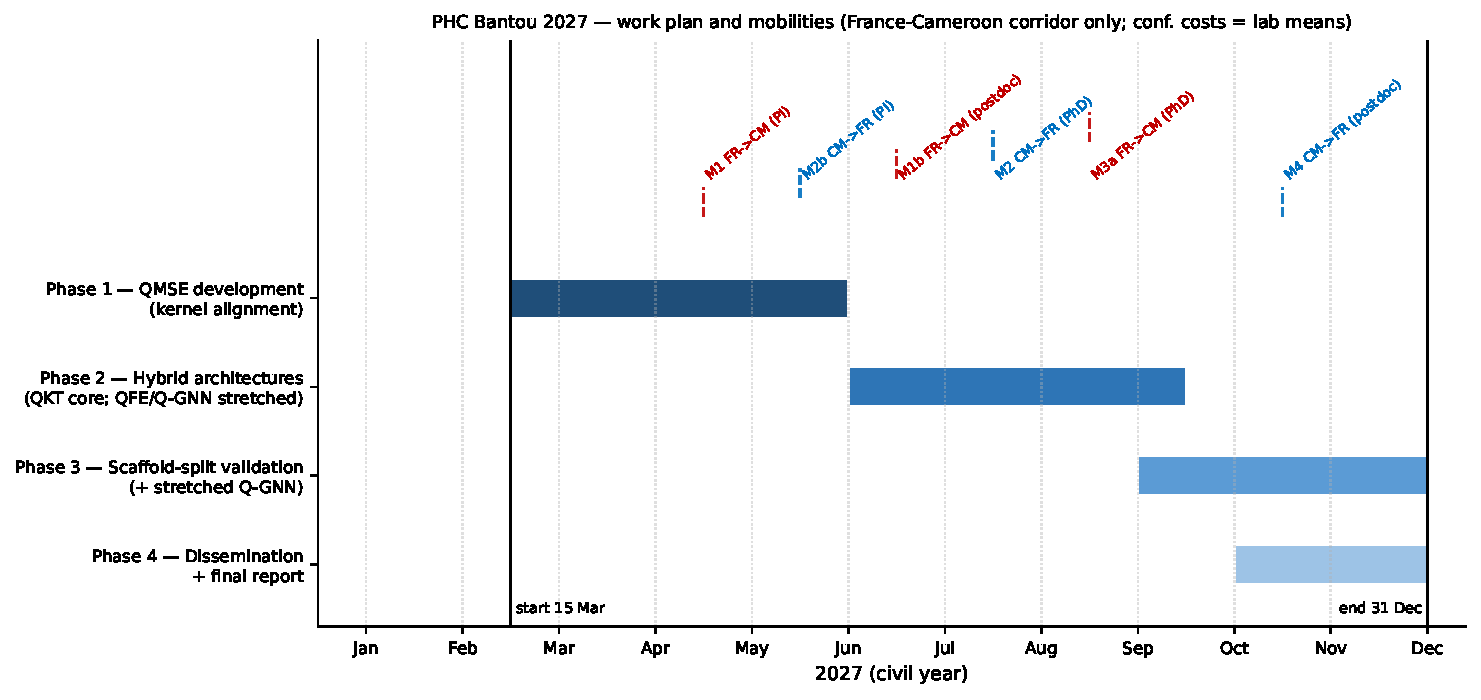
\includegraphics[width=0.95\textwidth]{figures/gantt_2027.pdf}
    \caption{Work plan 2027: four activity phases with mobility schedule (France--Cameroon corridor only). Red dashed lines: France $\rightarrow$ Cameroon mobilities (French envelope). Blue dashed lines: Cameroon $\rightarrow$ France mobilities (Cameroonian envelope, including PhD training). International conference costs are outside PHC Bantou (laboratory means).}
\label{fig:gantt}
\end{figure}

\subsubsection{Phase 1: QMSE Development (March--June 2027)}
\begin{itemize}
    \item Implement BondOrderMatrix and Coulomb-matrix encodings \cite{boy2025,rupp2012}
    \item Kernel alignment on Study 3 benchmark + ANP-rich subset; Set A feasibility demo
    \item \textbf{Mobility 1 (France $\rightarrow$ Cameroon, May 2027, 8 days):} PI FR (solo, senior rate window); joint algorithm design, WP-CM1 annotation kick-off
    \item \textbf{Mobility 2b (Cameroon $\rightarrow$ France, June 2027, 8 days):} PI CM (solo, senior rate window); QMSE design review, annotation-protocol kickoff (WP-CM1)
\end{itemize}

\subsubsection{Phase 2: Hybrid Architecture Training (July--October 2027)}
\begin{itemize}
    \item Train QKT (guaranteed core) on the frozen benchmark; QFE and Q-GNN as resources allow (stretched)
    \item ACSI-stratified evaluation (quartile analysis, Eq.\ \ref{eq:acsi})
    \item Hyperparameter optimization on simulators; hardware validation on a pre-declared subset only
    \item \textbf{Mobility 1b (France $\rightarrow$ Cameroon, July 2027, 15 days):} postdoctoral researcher FR (solo, junior rate window); architecture training review, WP-CM2 setup
    \item \textbf{Mobility 2 (Cameroon $\rightarrow$ France, August 2027, 21 days):} \textbf{Cameroonian PhD candidate (solo, junior rate window)} --- hands-on QML training, joint experiments, authorship workshops
    \item \textbf{Mobility 3a (France $\rightarrow$ Cameroon, September 2027, 21 days):} PhD candidate FR (solo, junior rate window); extended joint-analysis visit, ACSI annotation review, workshop facilitation
    \item Joint workshop ``Quantum Machine Learning for African Drug Discovery'' (September 2027, hosted in Cameroon during Mobility 3a; French PhD candidate on site, both full teams by videoconference; costs covered by laboratory means --- see \S\ref{sec:budget})
\end{itemize}

\subsubsection{Phase 3: External Validation (October--December 2027)}
\begin{itemize}
    \item Repeated scaffold-split validation on external set (protocol \S\ref{sec:data})
    \item FR/CM comparative performance report (WP-CM2)
    \item Feature attribution and interpretability analysis
    \item \textbf{Mobility 4 (Cameroon $\rightarrow$ France, November 2027, 15 days):} Cameroonian postdoctoral researcher (solo, junior rate window); hardware subset validation, manuscript drafting
\end{itemize}

\subsubsection{Phase 4: Dissemination and Final Reporting (November--December 2027, plus final report within 3 months after project end)}
\begin{itemize}
    \item Manuscript preparation; code repository release (GitHub) with documentation, subject to PPST check (\S\ref{sec:ethics})
    \item Final joint analysis meeting (December 2027, videoconference; no travel cost)
    \item Conference presentations at international meetings (ACS, EuroQCI, African computational-chemistry events) --- costs covered by laboratory means or other grants, not by PHC Bantou
    \item \textbf{Final scientific and financial report:} French PI files the Campus France report model via ECLECTUS within 3 months after project end; Cameroonian PI submits the MINRESI-format report; publications must acknowledge MEAE/MESRE/MINRESI and the project number
\end{itemize}

\subsection{Deliverables}

\textbf{Scientific Outputs:}
\begin{enumerate}
    \item Peer-reviewed manuscript on hybrid quantum-classical ML for ANP antimalarial prediction, with honest-negative reporting where applicable
    \item Open-source software package: \texttt{qml-anp} (Python, documented, BSD licence) --- deposited after PPST review
    \item Benchmark dataset: ANP-stratified antimalarial activity dataset with ACSI annotations, frozen manifests (SHA-256), DOI via Zenodo
    \item Technical report: simulator vs.\ hardware performance comparison (or explicit NOT\_COMPUTED statement if allocation is unavailable)
    \item \textbf{Final scientific and financial report} (Campus France model, $\leq$ 3 months after project end)
\end{enumerate}

\textbf{Training Outcomes:}
\begin{enumerate}
    \item \textbf{Joint supervision of 2 PhD candidates} (1 French, 1 Cameroonian; recruitment/registration in progress) --- PhD degrees are not expected within 12 months; the deliverable is the supervised research progress, co-authored outputs, and the training mobilities budgeted above
    \item Hands-on quantum-ML training for the Cameroonian PhD candidate via Mobility 2 (3 weeks in France, August 2027)
    \item Joint supervision framework established for future collaborations (co-tutelle pathway)
\end{enumerate}

\textbf{Capacity Building:}
\begin{enumerate}
    \item Workshop materials and tutorials on quantum computing for molecular modeling (costs: laboratory means)
    \item CPU-only deployment of \texttt{qml-anp} on Cameroonian institutional infrastructure (WP-CM2)
    \item French--Cameroonian quantum-computing working group, with explicit links to European networks (see \S\ref{sec:europe})
\end{enumerate}

\section{Budget Justification}
\label{sec:budget}

\textbf{Regulatory frame.} PHC Bantou funds cover \textbf{only} mobility between France and Cameroon of researchers (including PhD candidates and postdocs) belonging to \textbf{each team's own side}: the French envelope finances French-team travellers on France$\leftrightarrow$Cameroon trips; the Cameroonian envelope finances Cameroonian-team travellers on the same corridor. Third-country travel (e.g., international conferences outside the two countries) is \textbf{not} charged to PHC Bantou and is covered by laboratory means or other grants. Every other cost (computing, workshop materials, database curation, ethnobotanical field work, workshop hosting, conference registration) is covered by \textbf{laboratory means} and is presented below as assumed co-financing, outside the funds requested.

\textbf{Rate schedule (official Bantou table).} Senior researchers receive 125\,€/day for stays of \textbf{5 to 14 days}; PhD candidates and postdocs (junior researchers) receive 62\,€/day for stays of \textbf{15 to 30 days}; the air-ticket ceiling is \textbf{1,500\,€ per traveller} (budgeted here at 1,200\,€ per round-trip ticket, with a contingency line to the ceiling). Mobilities are therefore planned as \textbf{solo trips} (one traveller per mobility), and every line below is costed bottom-up as ticket + per diem $\times$ days. Co-investigators participate by videoconference at no PHC cost.

\subsection{French Team Budget ($\leq$ 7,500\,€ --- mobility only, France$\leftrightarrow$Cameroon)}

\begin{table}[htbp]
\centering
\small
\begin{tabular}{lrl}
\toprule
\textbf{Item} & \textbf{Cost (€)} & \textbf{Travellers / details} \\
\midrule
Mobility 1: France $\rightarrow$ Cameroon, May 2027 (8 days, senior) & 2,200 & PI FR, solo; airfare 1,200 + per diem $8\times125$ \\
Mobility 1b: France $\rightarrow$ Cameroon, Jul 2027 (15 days, junior) & 2,130 & Postdoc FR, solo; airfare 1,200 + per diem $15\times62$ \\
Mobility 3a: France $\rightarrow$ Cameroon, Sep 2027 (21 days, junior) & 2,402 & PhD candidate FR, solo; airfare 1,200 + per diem $21\times62$ \\
Airfare contingency (PHC ticket ceiling 1,500\,€) & 768 & fare variation buffer on the three tickets \\
\midrule
\textbf{Total France} & \textbf{7,500} & \textit{3 solo mobilities; French-team travellers only, FR$\leftrightarrow$CM} \\
\bottomrule
\end{tabular}
\end{table}

\subsection{Cameroonian Team Budget ($\leq$ 7,500\,€ --- mobility only, Cameroon$\leftrightarrow$France)}

\begin{table}[htbp]
\centering
\small
\begin{tabular}{lrl}
\toprule
\textbf{Item} & \textbf{Cost (€)} & \textbf{Travellers / details} \\
\midrule
Mobility 2b: Cameroon $\rightarrow$ France, Jun 2027 (8 days, senior) & 2,200 & PI CM, solo; airfare 1,200 + per diem $8\times125$ \\
Mobility 2: Cameroon $\rightarrow$ France, Aug 2027 (21 days, junior) & 2,402 & PhD candidate CM, solo; airfare 1,200 + per diem $21\times62$ \\
Mobility 4: Cameroon $\rightarrow$ France, Nov 2027 (15 days, junior) & 2,130 & Postdoc CM, solo; airfare 1,200 + per diem $15\times62$ \\
Airfare contingency (PHC ticket ceiling 1,500\,€) & 768 & fare variation buffer on the three tickets \\
\midrule
\textbf{Total Cameroon} & \textbf{7,500} & \textit{3 solo mobilities; Cameroonian-team travellers only, CM$\leftrightarrow$FR} \\
\bottomrule
\end{tabular}
\end{table}

\subsection{Co-financing by Laboratory Means (not requested from PHC)}

The following costs are real, budgeted by the partner laboratories, and explicitly \textbf{not} requested from PHC Bantou:

\begin{table}[htbp]
\centering
\small
\begin{tabular}{lrl}
\toprule
\textbf{Item} & \textbf{Indicative (€)} & \textbf{Covered by} \\
\midrule
Quantum/cloud computing and GPU hours & 800 & French laboratory \\
Workshop materials and tutorial datasets & 400 & French laboratory \\
ANP metadata curation and database governance & 800 & Cameroonian laboratory \\
Ethnobotanical field protocol (WP-CM4, ethics-approved) & 700 & Cameroonian laboratory \\
Workshop hosting (venue, local logistics) & 600 & Cameroonian laboratory \\
International conference registration/travel (outside FR--CM corridor) & 1,500 & Laboratory means / other grants \\
\midrule
\textbf{Subtotal co-financing} & \textbf{4,800} & \\
\bottomrule
\end{tabular}
\end{table}

Each partner team includes at least one PhD-candidate mobility, in line with the programme's emphasis on young researchers. All PHC-funded mobilities run on the France--Cameroon corridor between 15 March and 31 December 2027; engagement forms are filed $\geq$ 3 weeks before each departure; all funds are consumed before 31 December 2027.

\section{Expected Impact and Broader Significance}

\subsection{Scientific Impact}

\begin{enumerate}
    \item \textbf{Among the first genuine quantum-ML pipelines for ANP chemical space:} moving beyond quantum-inspired re-encodings of classical fingerprints \cite{havlicek2019,boy2025}
    \item \textbf{Honest assessment framework:} Establish standards for reporting quantum advantage, equivalence (TOST), and limitations in molecular ML \cite{lakens2017}
    \item \textbf{Scaffold generalization:} Address the 1-WL GNN bottleneck that limits classical methods on complex natural products \cite{morris2019}
    \item \textbf{Computational accessibility:} QKT enables ANP screening on modest resources (CPU-only), with the claim to be \textit{demonstrated} on Cameroonian infrastructure (WP-CM2)
\end{enumerate}

\subsection{Translational Impact}

\begin{enumerate}
    \item \textbf{Prioritized candidate list:} deliver a ranked, ACSI-annotated list of ANP-derived antimalarial candidates together with a ready-to-use experimental validation protocol (IC$_{50}$, resistance profiling) --- for a \textit{follow-on} project. This project itself has no experimental bioassay partner; it does not promise IC$_{50}$ data.
    \item \textbf{Traditional medicine:} provide computational evidence supporting ethnobotanical knowledge of antimalarial plants \cite{bero2009}, with benefit-sharing principles under the Nagoya Protocol \cite{nagoya2011}
    \item \textbf{Sustainable drug discovery:} open, reusable framework for ongoing ANP exploration using African botanical resources
    \item \textbf{Regional health relevance:} focus on compounds and targets aligned with African \textit{Plasmodium} resistance profiles
\end{enumerate}

\subsection{Capacity Building Impact}

\begin{enumerate}
    \item \textbf{Quantum computing expertise in Africa:} train the next generation of African quantum researchers on a concrete health priority; Mobilities 2 and 3a are dedicated PhD-training mobilities
    \item \textbf{Franco-Cameroonian network:} sustained collaboration beyond this call (co-tutelle, follow-on proposals, student exchanges)
    \item \textbf{Infrastructure:} roadmap + actual CPU-only deployment for computational chemistry / quantum-ML workflows in Cameroonian institutions
    \item \textbf{Regional dissemination:} workshop and software package designed for pan-African adoption
\end{enumerate}

\subsection{Cultural and Ethical Dimensions}

\begin{enumerate}
    \item \textbf{Honoring traditional knowledge:} explicit acknowledgment of ethnobotanical heritage and traditional medicine practitioners; ethics-governed field protocol (\S\ref{sec:ethics})
    \item \textbf{Equitable collaboration:} joint authorship, co-supervision, Cameroonian-led annotation governance, shared IP following Nagoya principles \cite{nagoya2011}
    \item \textbf{Benefit sharing:} if ANP-derived candidates advance to development, mechanisms for benefit sharing with source communities
    \item \textbf{Open science:} code, data, and methods openly shared after PPST review, enabling global participation
\end{enumerate}

\section{Risk Management}
\label{sec:risk}

\subsection{Technical Risks}

\textbf{Risk 1: Quantum hardware limitations (NISQ noise)}
\begin{itemize}
    \item Mitigation: extensive simulator validation, error mitigation protocols, hybrid quantum-classical fallback \cite{preskill2018}
    \item Contingency: focus on QKT (fewer quantum operations) if full Q-GNN training infeasible on current hardware
\end{itemize}

\textbf{Risk 2: Quantum equivalence outcome (no advantage over ECFP4)}
\begin{itemize}
    \item Mitigation: following Study 3 precedent, equivalence is a valid scientific result (tested by TOST \cite{lakens2017}); focus on identifying \textit{when} quantum helps vs.\ when classical methods suffice
    \item Impact: still publishable (honest-negative framework), still provides value to the field
\end{itemize}

\textbf{Risk 3: Scope stretch (Q-GNN and 10k external validation)}
\begin{itemize}
    \item Mitigation: \textbf{guaranteed scope = Aim 1 + Aim 3 + the QKT architecture of Aim 2} (QMSE, ACSI stratification, quantum-kernel transfer); QFE/Q-GNN training and the full 10k validation are pre-declared \textit{stretched} objectives
    \item Contingency: scale down external validation if resources run short; HPO remains on simulators; hardware validation is a pre-declared subset
\end{itemize}

\textbf{Risk 4: IBM Quantum allocation not granted in time}
\begin{itemize}
    \item Mitigation: cloud allocation application submitted at project start; all core estimands computable on simulators
    \item Contingency: report hardware validation as NOT\_COMPUTED with full transparency; do not improvise alternative claims
\end{itemize}

\subsection{Logistical Risks}

\textbf{Risk 5: Travel restrictions or delays}
\begin{itemize}
    \item Mitigation: buffer dates for each mobility; engagement forms filed $\geq$ 3 weeks ahead; November schedule leaves margin before 31 December
    \item Contingency: virtual collaboration tools (weekly video meetings, shared compute clusters, Git-based workflows)
\end{itemize}

\textbf{Risk 6: Data access or licensing issues}
\begin{itemize}
    \item Mitigation: all primary databases (AfroDb, ANPDB, ChEMBL) are freely downloadable \cite{ntiekang2013,mendez2019}; no licence fee is budgeted or expected
    \item Contingency: use public datasets with ANP filters; co-financing by laboratory means covers curation
\end{itemize}

\textbf{Risk 7: PhD recruitment timeline}
\begin{itemize}
    \item Mitigation: recruitment/registration started before the call; if delayed, mobilities are reassigned to co-I/postdoc travellers without exceeding envelope caps
\end{itemize}

\section{Dissemination, Open Science, and European Integration}
\label{sec:europe}

\subsection{Publications and Presentations}

\begin{enumerate}
    \item Primary manuscript: computational chemistry / molecular-ML journal (\textit{RSC Digital Discovery} as first target, given the project's computational open-science profile; \textit{JCIM}, \textit{JCAMD} as alternates)
    \item Conference presentations: ACS Fall Meeting, EuroQCI quantum-chemistry workshops, African computational-chemistry meetings --- costs covered by laboratory means or other grants (not PHC Bantou)
    \item Preprint: arXiv or ChemRxiv for rapid dissemination and community feedback
\end{enumerate}

\subsection{Open Science Commitments}

\begin{enumerate}
    \item Code: GitHub repository with BSD licence, continuous integration, documentation --- deposited after PPST review (\S\ref{sec:ethics})
    \item Data: Zenodo deposition with DOI (activity data, ACSI annotations, frozen manifests with SHA-256, trained model weights)
    \item Reproducibility: container images (Docker/Singularity) for full pipeline reproduction
    \item Tutorial: Jupyter notebooks demonstrating QMSE encoding and QKT workflow
    \item All publications must acknowledge MEAE/MESRE/MINRESI and the PHC project number
\end{enumerate}

\subsection{European Integration and Structuring}

European integration is a stated priority of the PHC Bantou call. This project is designed to plug into European quantum and health networks from day one:

\begin{itemize}
    \item \textbf{EuroQCI / Quantum Europe:} joint attendance and contribution to EuroQCI-related quantum-chemistry workshops; the French team will pursue EuroQCI-affiliated events through the conference slot and hybrid participation
    \item \textbf{Horizon Europe alignment:} the topic sits at the intersection of Cluster 4 (digital, industry, space --- quantum technologies) and Cluster 1 (health); follow-on proposals will target Horizon Europe collaborative calls, with the PHC Bantou collaboration as the proven bilateral base
    \item \textbf{ANR--MINRESI and other bilateral calls:} the same theme may be resubmitted to other PHC/Bantou-type bilateral programmes, which the programme explicitly allows
    \item \textbf{Regional network:} collaboration with other African quantum initiatives (South Africa NQI, Egypt QCI) through the French team's European networks
\end{itemize}

\subsection{Long-Term Collaboration}

This PHC Bantou project establishes the foundation for:
\begin{itemize}
    \item PhD co-supervision programs (joint degrees, sandwich programs) --- initiated for the two PhD candidates (recruitment in progress)
    \item Follow-on proposals: Horizon Europe, ANR--MINRESI bilateral calls, African Union research grants
    \item Experimental validation partnerships: synthesis and bioassay of top-ranked ANP candidates in a subsequent project
    \item Regional network expansion: pan-African quantum-ML-for-health working group
\end{itemize}

\section{Team Composition and Expertise}

\textit{[Author note --- not for ECLECTUS: fields marked \texttt{[TO COMPLETE]} must be filled with real names, institutions, and up to five publications before submission. ECLECTUS team fields are structured forms, not free text.]}

\subsection{French Team}

\textbf{Principal Investigator:} \texttt{[TO COMPLETE --- name, position, institution]}
\begin{itemize}
    \item Expertise: quantum machine learning, computational chemistry, molecular modeling
    \item Role: overall project coordination, quantum algorithm development, manuscript preparation
    \item Relevant publications (max.\ 5 for ECLECTUS): \texttt{[TO COMPLETE]}
\end{itemize}

\textbf{Co-Investigators:} \texttt{[TO COMPLETE --- names, positions]}
\begin{itemize}
    \item Quantum computing specialist: IBM Quantum access, circuit optimization, error mitigation
    \item Machine learning expert: neural network architectures, hyperparameter tuning, feature attribution
    \item Computational chemist: molecular dynamics, docking, QSAR modeling
\end{itemize}

\textbf{PhD candidate (1):} \texttt{[TO COMPLETE --- name, enrolment status]}
\begin{itemize}
    \item Profile: computational chemistry or physics background, interest in quantum ML
    \item Training: quantum computing, ANP drug discovery, Franco-African collaboration skills
\end{itemize}

\textbf{Postdoctoral researcher (1):} \texttt{[TO COMPLETE --- name, institution]}

\subsection{Cameroonian Team}

\textbf{Principal Investigator:} \texttt{[TO COMPLETE --- name, position, institution]}
\begin{itemize}
    \item Expertise: natural products chemistry, ethnobotany, traditional medicine
    \item Role: ANP database governance, ethnobotanical validation, local coordination, WP-CM1/WP-CM4 leadership
    \item Relevant experience (max.\ 5 productions for ECLECTUS): \texttt{[TO COMPLETE]}
\end{itemize}

\textbf{Co-Investigators:} \texttt{[TO COMPLETE --- names, positions]}
\begin{itemize}
    \item Ethnobotanist: traditional antimalarial plant knowledge, botanical specimen identification
    \item Computational chemist: molecular modeling, cheminformatics, database management, WP-CM2 lead
    \item Public health specialist: malaria epidemiology, resistance patterns in Cameroon
\end{itemize}

\textbf{PhD candidate (1):} \texttt{[TO COMPLETE --- name, enrolment status]}
\begin{itemize}
    \item Profile: chemistry or biology background, strong computational interest
    \item Training: quantum machine learning (Mobility 2), computational drug discovery, co-authorship on publications
\end{itemize}

\subsection{History of Franco-Cameroonian Cooperation}

\textit{[Author note --- ECLECTUS field ``Rappel du contexte de la coopération et des relations existantes entre les 2 équipes'' is mandatory. TO COMPLETE with: date and setting of first meeting; previous visits; joint publications; letters of support; ongoing co-supervision. A draft skeleton:]}
\begin{itemize}
    \item First contact: \texttt{[TO COMPLETE --- year, venue]}
    \item Previous mobility/exchange: \texttt{[TO COMPLETE]}
    \item Joint publications to date: \texttt{[TO COMPLETE --- up to 5]}
    \item Letters of support: \texttt{[TO COMPLETE --- from both host institutions]}
\end{itemize}

\section{Alignment with PHC Bantou Priorities}

This proposal strongly aligns with the PHC Bantou programme objectives:

\begin{enumerate}
    \item \textbf{Excellence in scientific cooperation:} merges frontier quantum computing with an urgent African health challenge (malaria), leveraging complementary French--Cameroonian strengths
    \item \textbf{New collaborations:} establishes a novel partnership in quantum ML for natural products, beyond traditional chemistry-only or computation-only collaborations
    \item \textbf{Young researcher participation:} central role for PhD candidates --- two dedicated PhD mobilities (Mobilities 2 and 3a), hands-on training, co-authorship
    \item \textbf{Structuring and valorisation:} sustainable framework (open-source tools, training materials, joint supervision) with a clear translational path (prioritized ANP antimalarial candidates for a follow-on experimental project)
    \item \textbf{European integration:} EuroQCI engagement, Horizon Europe Cluster 1/4 alignment, follow-on EU proposals (\S\ref{sec:europe})
    \item \textbf{Computational accessibility:} QKT explicitly designed for resource-limited settings; the claim is demonstrated, not asserted, through WP-CM2 local deployment
\end{enumerate}

\section{Conclusion}

This Franco-Cameroonian collaboration addresses a critical scientific challenge (antimalarial drug discovery from African natural products) using frontier computational methods (hybrid quantum-classical machine learning) while building sustainable research capacity in Africa. By moving beyond quantum-inspired approaches to genuine quantum-computing applications, we will determine when and how quantum enhancement benefits structurally complex natural products that defeat classical methods --- with pre-declared estimands, repeated-split statistics, TOST equivalence testing, and honest-negative reporting.

Our approach is grounded in rigorous preliminary work (Studies 1--5), keeps the guaranteed scope realistic for the project period and the available means (Aim 1 + Aim 3 + QKT; QFE/Q-GNN training and the 10k validation as pre-declared stretched objectives), and prioritizes genuine two-way complementarity: Cameroonian-led annotation governance, local CPU-only deployment, and PhD training mobilities. The project honors traditional African medicine knowledge, creates opportunities for young Franco-Cameroonian researchers, and establishes the foundation for long-term collaboration in quantum computing for health applications.

We respectfully request PHC Bantou support to launch this partnership and advance quantum machine learning for African natural-product drug discovery.

\vspace{1em}
\noindent\textit{[Post-selection acknowledgment template --- insert only after selection:] This project is supported by the ``PHC BANTOU'' program, funded by the French Ministry for Europe and Foreign Affairs (MEAE), the French Ministry for Higher Education, Research and Space (MESRE), and the Cameroonian Ministry for Scientific Research and Innovation (MINRESI) [project number: XXXXXXX].}

\clearpage

\section*{Internal Note --- ECLECTUS Submission Procedure (remove before any circulation as final proposal)}

\begin{itemize}
    \item \textbf{Platform:} the application is filed exclusively on ECLECTUS. There is no paper/PDF dossier per se; this LaTeX/PDF document is the drafting matrix.
    \textbf{Initiation:} the \textbf{French partner initiates} the application and invites the Cameroonian partner via the platform.
    \textbf{Only the French partner submits} the final application.
    \textbf{Deadline:} 29 October 2026. Initiate by 22 October 2026 at the latest.
    \textbf{Text fields:} each of the four narrative fields is capped at 10,000 characters (spaces + line breaks + paragraphs included). Use \texttt{Bantou\_2027\_formfields.md} for the compressed drafts.
    \textbf{Attachments:} JPG/GIF/PNG/PDF (unprotected) only.
    \textbf{Teams:} structured forms for French and Cameroonian teams; fill real names and $\leq$ 5 productions each.
    \textbf{Confirm with MINRESI focal point} whether a parallel national filing is required (the call text mentions co-deposit in each country).
    \textbf{File this project's engagement forms} $\geq$ 3 weeks before each mobility departure.
    \textbf{Final report:} French PI files the Campus France model via ECLECTUS $\leq$ 3 months after 31 December 2027; Cameroonian PI submits the MINRESI-format report; publications must cite MEAE/MESRE/MINRESI + project number.
\end{itemize}

\clearpage
\phantomsection
\addcontentsline{toc}{section}{References}
\begin{thebibliography}{20}
\bibitem{who2025}
World Health Organization.
\textit{World Malaria Report 2025}.
Geneva: WHO; 2025.
ISBN 9789240117822.
Available at: \url{https://www.who.int/publications/i/item/9789240117822} (accessed 6 October 2026).

\bibitem{ntiekang2013}
Ntie-Kang F, Zofou D, Babiaka SB, et al.
AfroDb: A select highly potent and diverse natural product library from African medicinal plants.
\textit{PLoS ONE}. 2013;8(9):e78085.
doi:10.1371/journal.pone.0078085.

\bibitem{lovering2009}
Lovering F, Bikker J, Humblet C.
Escape from Flatland: increasing saturation as an opportunity to modulate complexity.
\textit{J Med Chem}. 2009;52(21):6752--6756.
doi:10.1021/jm901241e.

\bibitem{bemis1996}
Bemis GW, Murcko MA.
The properties of known drugs. 1. Molecular frameworks.
\textit{J Med Chem}. 1996;39(15):2887--2893.
doi:10.1021/jm9602928.

\bibitem{rogers2010}
Rogers D, Hahn M.
Extended-connectivity fingerprints.
\textit{J Chem Inf Model}. 2010;50(5):742--754.
doi:10.1021/ci100050t.

\bibitem{morris2019}
Morris C, Ritzert M, Fey M, et al.
Weisfeiler and Leman go neural: higher-order graph neural networks.
In: \textit{Proceedings of the AAAI Conference on Artificial Intelligence}. 2019;33:4602--4609.
doi:10.1609/aaai.v33i01.33014602.

\bibitem{wu2018}
Wu Z, Ramsundar B, Feinberg EN, et al.
MoleculeNet: a benchmark for molecular machine learning.
\textit{Chem Sci}. 2018;9:513--530.
doi:10.1039/C7SC02664A.

\bibitem{rupp2012}
Rupp M, Tkatchenko A, M\"uller K-R, von Lilienfeld OA.
Fast and accurate modeling of molecular atomization energies with machine learning.
\textit{Phys Rev Lett}. 2012;108:058301.
doi:10.1103/PhysRevLett.108.058301.

\bibitem{havlicek2019}
Havl\'{i}\v{c}ek V, C\'{o}rcoles AD, Temme K, et al.
Supervised learning with quantum-enhanced feature spaces.
\textit{Nature}. 2019;567:209--212.
doi:10.1038/s41586-019-0980-2.

\bibitem{boy2025}
Boy C, Altamura E, Manawadu D, et al.
Encoding molecular structures in quantum machine learning.
\textit{Mach Learn: Sci Technol}. 2025;6(4):045076.
doi:10.1088/2632-2153/ae304f.

\bibitem{preskill2018}
Preskill J.
Quantum computing in the NISQ era and beyond.
\textit{Quantum}. 2018;2:79.
doi:10.22331/q-2018-08-06-79.

\bibitem{kim2023}
Kim Y, Eddins A, Anand S, et al.
Evidence for the utility of quantum computing before fault tolerance.
\textit{Nature}. 2023;618:500--505.
doi:10.1038/s41586-023-06096-3.

\bibitem{mcnutt2021}
McNutt AT, Francoeur P, Aggarwal R, et al.
GNINA 1.0: molecular docking with deep learning.
\textit{J Cheminform}. 2021;13:13.
doi:10.1186/s13321-021-00522-2.

\bibitem{bauer2013}
Bauer M, Ibrahim T, Vogel S, et al.
Evaluation and optimization of virtual screening workflows with DEKOIS 2.0.
\textit{J Chem Inf Model}. 2013;53(6):1447--1462.
doi:10.1021/ci400115b.

\bibitem{mendez2019}
Mendez D, Gaulton A, Bento AP, et al.
ChEMBL: towards direct deposition of bioassay data.
\textit{Nucleic Acids Res}. 2019;47(D1):D930--D940.
doi:10.1093/nar/gky1075.

\bibitem{lakens2017}
Lakens D.
Equivalence tests: a practical primer for t tests, correlations, and meta-analyses.
\textit{Soc Psychol Pers Sci}. 2017;8(4):355--362.
doi:10.1177/1948550617697177.

\bibitem{delong1988}
DeLong ER, DeLong DM, Clarke-Pearson DL.
Comparing the areas under two or more correlated receiver operating characteristic curves: a nonparametric approach.
\textit{Biometrics}. 1988;44(3):837--845.
doi:10.2307/2531595.

\bibitem{bero2009}
Bero J, Fr\'{e}d\'{e}rich M, Quetin-Leclercq J.
Antimalarial compounds isolated from plants used in traditional medicine.
\textit{J Pharm Pharmacol}. 2009;61(11):1401--1433.
doi:10.1211/jpp.61.11.0001.

\bibitem{nagoya2011}
Convention on Biological Diversity.
\textit{Nagoya Protocol on Access to Genetic Resources and the Fair and Equitable Sharing of Benefits Arising from Their Utilization to the Convention on Biological Diversity}.
UNEP/CBD/COP/DEC/X/20; 2011.
Available at: \url{https://www.cbd.int/abs/text} (accessed 6 October 2026).

\end{thebibliography}

\end{document}
